\section{Introduction to ZX-Calculus}

As stated in the previous section, the ZX-Calculus is represented by the
$\mathbf{FDHilb}$ category, meaning that the objects of our category are finite-dimensional Hilbert spaces, and the morphisms are linear maps between those Hilbert spaces. The morphisms will be represented using the so-called $\textit{Spiders}$. This means that the whole classical quantum circuit will be represented by a network of morphism/spiders. This representation is advantageous, as it allows for a straightforward application of the simplification rules we will define later.

\subsection{Spiders}

Spiders are the $\textit{atoms}$ of a ZX-Diagram. They represent the decomposition of quantum gates into even smaller and more fundamental operations.
Spiders can have an arbitrary number of incoming and outgoing edges and appear in two flavors: $\textit{Z-Spiders}$ and $\textit{X-Spiders}$. This distinction is shown visually using the green and red colors when drawing the spiders.
Additionally, spiders may carry a phase value $\alpha \in [0, 2\pi)$, which can be omitted if the angle is zero.

The spiders are shown visually in figure \ref{fig:spiders-visual}. The left spider is a $\textit{Z-Spider}$, and the right one is an $\textit{X-Spider}$. Both have $n$ incoming and $m$ outgoing edges, carrying a phase value $\alpha$.

\begin{figure}[h]
    \centering
    \begin{align*}
        \underbrace{
            \begin{ZX}
                \leftManyDots{n}  \zxZ{\alpha} \rightManyDots{m}
            \end{ZX}
        }_{\text{Z-Spider}}
        \qquad
        \underbrace{
            \begin{ZX}
                \leftManyDots{n}  \zxX{\alpha} \rightManyDots{m}
            \end{ZX}
        }_{\text{X-Spider}}
    \end{align*}
    \caption{Fundamental spiders with $n$ incoming and $m$ outgoing edges, carrying a phase value $\alpha$}
    \label{fig:spiders-visual}
\end{figure}


It is important to remember that each spider represents a morphism in the $\mathbf{FDHilb}$ category. Therefore, each spider represents a linear map from the incoming $n$ to the outgoing $m$ qubits. Those linear maps can be calculated explicitly and are shown in figure \ref{fig:individual-spiders-linear-maps}. We will use the notation $\left \llbracket \cdot \right \rrbracket$ to denote the linear map represented by a spider.

\begin{figure}
    \begin{align*}
        \left \llbracket
        \begin{ZX}
            \leftManyDots{n}  \zxZ{\alpha} \rightManyDots{m}
        \end{ZX}
        \right \rrbracket
        := & |\underbrace{0\dots 0}_{m}\rangle \langle \underbrace{0\dots0}_{n}| + e^{i\alpha}|\underbrace{1\dots1}_{m}\rangle \langle \underbrace{1\dots1}_{n}|
        \\
        =  & \begin{pmatrix}
                 1      & 0      & \dots  & 0           \\
                 0      & 0      & \dots  & 0           \\
                 \vdots & \vdots & \ddots & \vdots      \\
                 0      & 0      & \dots  & e^{i\alpha} \\
             \end{pmatrix}
        \\
        \left \llbracket
        \begin{ZX}
            \leftManyDots{n}  \zxX{\alpha} \rightManyDots{m}
        \end{ZX}
        \right \rrbracket
        := & |\underbrace{+ \dots +}_{m}\rangle \langle \underbrace{+ \dots +}_{n}| + e^{i\alpha}|\underbrace{- \dots -}_{m}\rangle \langle \underbrace{- \dots -}_{n}|
        \\
    \end{align*}
    \caption{Linear maps represented by individual spiders}
    \label{fig:individual-spiders-linear-maps}
\end{figure}


Note that the linear maps in figure \ref{fig:individual-spiders-linear-maps} do not have to be unitary, nor do they have to be square. The dimension of the linear map depends only on the number of incoming and outgoing edges. For example, a spider with $n$ incoming and $m$ outgoing edges represents a linear map in $\mathbb{C}^{2^m \times 2^n}$.

\subsection{Classical Quantum Gates as Spiders}

\begin{figure}[h]
    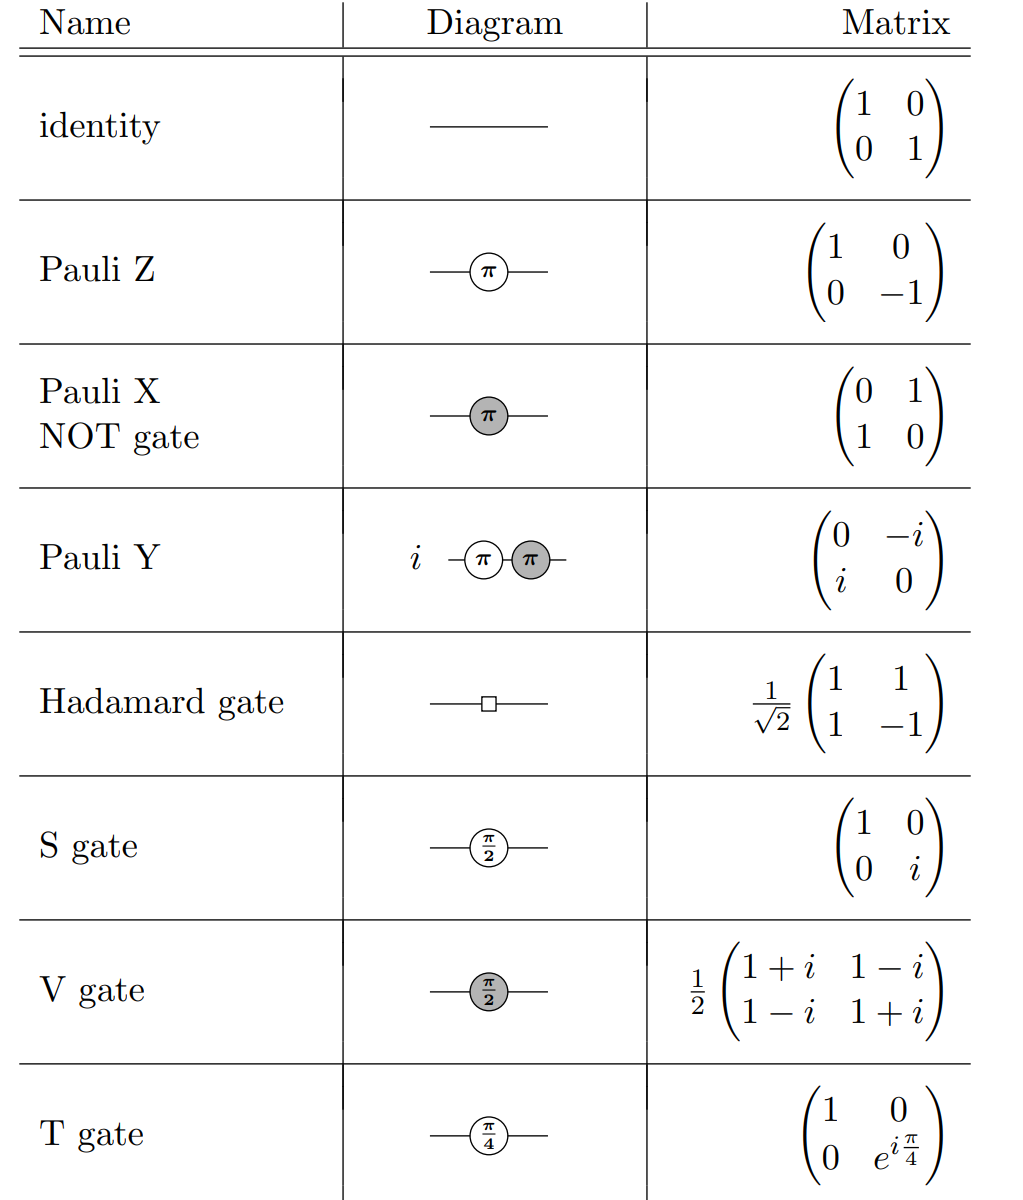
\includegraphics[width=\linewidth]{images/single_spider_unitaries.png}
    \caption{Spiders representing quantum gates
            {\cite{vandewetering2020zxcalculus}[P.87]}}
    \label{fig:spiders-gate-representation}
\end{figure}

By using the single spiders shown in figure \ref{fig:spiders-visual} we can already represent a lot of quantum gates. The most important ones are shown in figure \ref{fig:spiders-gate-representation}. We will ignore the global scalar values of ZX-Diagrams in the following sections since they are negligible for most calculations \cite{equivalence_checking_tum}. Furthermore, when working with unitary circuits, the scalar value can be restored at the end of the analysis as the resulting circuit matrix can be related to the unitary matrix \cite{vandewetering2020zxcalculus}.

It is easy to verify that the gates from figure \ref{fig:spiders-gate-representation} can be represented using just the basic spiders. This proof boils down to just inserting the corresponding spiders into the formulas from figure \ref{fig:individual-spiders-linear-maps} and comparing the resulting matrices with the matrices of the Pauli gates.
These proofs are shown in the Appendix in sections \ref{appendix:pauli-z-gate-as-spider}, \ref{appendix:pauli-x-gate-as-spider} and \ref{appendix:pauli-y-gate-as-spider}.

\subsection{Bigger Circuits}

Using the rules from figure \ref{fig:spiders-gate-representation} we can only represent circuits consisting of a single gate. For more extensive circuits, we need to combine multiple spiders into a single diagram. This is done by connecting the different spiders leg to leg. In particular, this means that one spider's outgoing leg connects to another spider's incoming legs.

But before working with such circuits, we need to define more rules to calculate the matrix representation of such a composed circuit.

\begin{enumerate}

    \item \textbf{Only Topology Matters}

          The first rule is that we can move spiders around freely if we maintain the correct order of the incoming and outgoing legs. This rule corresponds to the $\textit{Only Topology Matters}$ mantra of the ZX-Calculus and is justified by similar operations in the underlying $\mathbf{FDHilb}$-category.

    \item \textbf{Parallel Composition}

          The second rule allows us to calculate the matrix representation of spiders acting in parallel. We have seen this rule before when we looked at the category representation of parallel morphisms (\ref{parallel-composition}). In $\mathbf{FDHilb}$, this rule corresponds to taking the Kroncker product of the matrices of the \textit{parallel} spiders.

    \item \textbf{Sequential Composition}

          The third rule allows us to calculate the matrix representation of spiders acting in sequence. This rule corresponds to the sequential composition (\ref{sequential-composition}) in the category representation of the ZX-Calculus. In particular, it states that the composed linear map can be calculated by multiplying the individual spiders' matrices.
\end{enumerate}

\subsection{Example: CNOT Gate}

An example of a circuit consisting of multiple spiders is the classical \textbf{CNOT} gate, represented by the ZX-Diagram shown in figure \ref{fig:cnot-gate-split}.

To calculate this circuit's matrix representation, we must first split the ZX-Diagram into regions consisting of individual spiders. The result of this splitting is already shown in figure \ref{fig:cnot-gate-split-4}.

\begin{figure}
    \centering
    \subfloat[\centering CNOT split into 4 Regions\label{fig:cnot-gate-split-4}]{{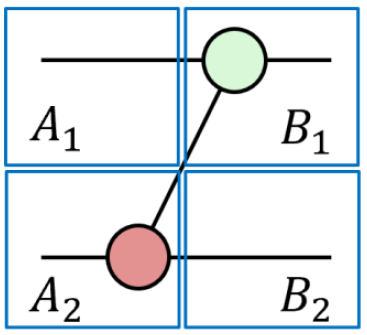
\includegraphics[height=3.5cm]{images/cnot-regions-4.png} }}
    \qquad
    \subfloat[\centering CNOT split into 2 Regions\label{fig:cnot-gate-split-2}]{{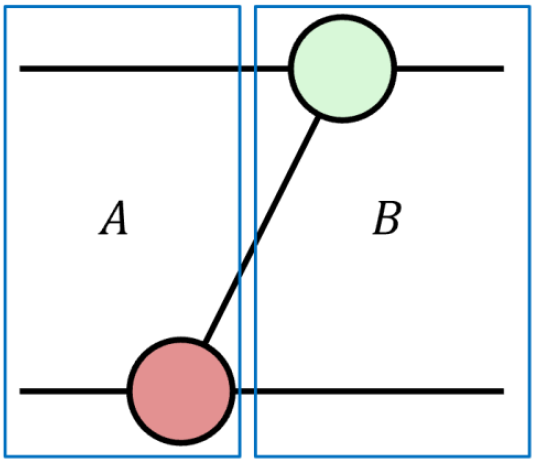
\includegraphics[height=3.5cm]{images/cnot-regions-2.png} }}
    \caption{Splitting the CNOT gate into regions}
    \label{fig:cnot-gate-split}
\end{figure}

Using the rules we just defined, we can now calculate the matrix representation of the circuit. We apply the $\textit{Parallel Composition}$ rule to combine sections $A_1$ and $A_2$ into a new section $A$. The same is done for sections $B_1$ and $B_2$, respectively. This reduction results in the ZX-Diagram shown in figure \ref{fig:cnot-gate-split-2}.

We can also write this calculation using a decomposition formula: Let $R$ be the matrix representation of the circuit shown in figure \ref{fig:cnot-gate-split-4}. Then we can write the reduction as shown in equation \ref{eq:cnot-gate-reduction}. All elements of the decomposition are individual spiders, so we can easily calculate their matrix representation using the rules from figure \ref{fig:individual-spiders-linear-maps}.


\begin{equation}
    \label{eq:cnot-gate-reduction}
    \begin{split}
        \underbrace{
            \left \llbracket
            \begin{ZX}
                \zxNone{} \rar & \zxNone{} \rar      & \zxZ{}\rar & \\
                \zxNone{} \rar & \zxX{} \rar \ar[ru] & \rar       & \\
            \end{ZX}
            \right \rrbracket
        }_{R}
        & =
        \underbrace{
            \left \llbracket
            \begin{ZX}
                \zxNone{} \rar & \zxNone{}\rar & \zxNone{} \\
                \zxNone{} \rar & \zxX{} \rar \ar[ru] & \zxNone{} \\
            \end{ZX}
            \right \rrbracket
        }_{A}
        \circ
        \underbrace{
            \left \llbracket
            \begin{ZX}
                \zxNone{} \rar      & \zxZ{}\rar & \\
                \zxNone{} \rar \ar[ru] & \rar       & \\
            \end{ZX}
            \right \rrbracket}_{B} \\
        & =
        (
        \underbrace{
            \left \llbracket
            \begin{ZX}
                \zxNone{} \rar & \zxNone{}\rar &[\zxwCol]  \zxNone{} \\
            \end{ZX} \right \rrbracket
        }_{A_1}
        \otimes
        \underbrace{
            \left    \llbracket
            \begin{ZX}
                \rar & \zxX{} \rightManyDots[0][0]{}
            \end{ZX}
            \right \rrbracket
        }_{A_2}
        )
        \circ
        (
        \underbrace{
            \left \llbracket
            \begin{ZX}
                \leftManyDots[0][0]{} \zxZ{} \rar & \zxNone{}
            \end{ZX}
            \right \rrbracket
        }_{B_1}
        \otimes
        \underbrace{
            \left    \llbracket
            \begin{ZX}
                \zxNone{} \rar & \zxNone{}\rar &[\zxwCol]  \zxNone{} \\
            \end{ZX}
            \right \rrbracket
        }_{B_2}
        )
    \end{split}
\end{equation}


The concrete calculation looks as follows:


\begin{align*}
    A    & = A_1 \otimes A_2                      \\
         & = id \otimes \left \llbracket
    \zx{
    \rar & \zxX{} \rightManyDots[0][0]{}
    } \right \rrbracket                           \\
         & =id    \otimes
    |+\rangle \langle ++| + |-\rangle \langle --| \\
         & = \begin{pmatrix}
                 1 & 0 \\
                 0 & 1 \\
             \end{pmatrix}
    \otimes
    \frac{1}{\sqrt{2}}
    \begin{pmatrix}
        1 & 0 \\
        0 & 1 \\
        0 & 1 \\
        1 & 0 \\
    \end{pmatrix}                                \\
         & = \frac{1}{\sqrt{2}}
    \begin{pmatrix}
        1 & 0 & 0 & 0 \\
        0 & 1 & 0 & 0 \\
        0 & 1 & 0 & 0 \\
        1 & 0 & 0 & 0 \\
        0 & 0 & 1 & 0 \\
        0 & 0 & 0 & 1 \\
        0 & 0 & 0 & 1 \\
        0 & 0 & 1 & 0 \\
    \end{pmatrix}
\end{align*}

\begin{align*}
    B                                 & = B_1 \otimes B_2               \\
                                      & =\left \llbracket \zx{
    \leftManyDots[0][0]{} \zxZ{} \rar & \zxNone{}
    } \right \rrbracket \otimes id                                      \\
                                      & =
    \begin{pmatrix}
        1 & 0 & 0 & 1 \\
        0 & 1 & 1 & 0 \\
    \end{pmatrix}
    \otimes
    \begin{pmatrix}
        1 & 0 \\
        0 & 1 \\
    \end{pmatrix}                                                      \\
                                      & = \begin{pmatrix}
                                              1 & 0 & 0 & 1 & 0 & 0 & 0 & 0 \\
                                              0 & 1 & 1 & 0 & 0 & 0 & 0 & 0 \\
                                              0 & 0 & 0 & 0 & 1 & 0 & 0 & 1 \\
                                              0 & 0 & 0 & 0 & 0 & 1 & 1 & 0 \\
                                          \end{pmatrix}
\end{align*}


Using the the $\textit{Sequential Composition}$ rule we can combine sections $A$ and $B$ into the resulting matrix $R$:

\begin{align*}
    R & = A \circ B         \\
      & = B \cdot A         \\
      & =
    \frac{1}{\sqrt{2}}
    \begin{pmatrix}
        1 & 0 & 0 & 0 \\
        0 & 1 & 0 & 0 \\
        0 & 0 & 0 & 1 \\
        0 & 0 & 1 & 0 \\
    \end{pmatrix}          \\
      & \propto \text{CNOT}
\end{align*}

The resulting matrix $R$ is proportional to the matrix representation of the CNOT gate. Therefore we showed that the ZX-Diagram \zx{
    \zxNone{} \rar & \zxNone{} \rar  &\zxZ{}\rar  &\\
    \zxNone{} \rar & \zxX{} \rar \ar[ru]  &\rar& \\
} is indeed a valid representation of the CNOT gate.


